\definecolor{dkgreen}{rgb}{0,0.6,0}
\definecolor{gray}{rgb}{0.5,0.5,0.5}
\definecolor{mauve}{rgb}{0.58,0,0.82}
\lstset{
  language=C++,
  aboveskip=3mm,
  belowskip=3mm,
  showstringspaces=false,
  columns=flexible,
  basicstyle={\fontsize{7}{9}\ttfamily},
  numbers=none,
  numberstyle=\tiny\color{gray},
  keywordstyle=\color{blue},
  commentstyle=\color{dkgreen},
  stringstyle=\color{mauve},
  breaklines=true,
  breakatwhitespace=true,
  tabsize=3
}

% ------------------------------------------------------------------------
\chapter{Simulator Structure}

\begin{refsection}



LinkPlanner is a signals open-source simulator.

The major entity is the system.

A system comprises a set of blocks.

The blocks interact with each other through signals.

\section{System}

\section{Blocks}

\section{Signals}

List of available signals:

\begin{itemize}
    \item Signal

\end{itemize}

\subsubsection{PhotonStreamXY}
A single photon is described by two amplitudes $A_x$ and $A_y$ and a phase difference between them, $\delta$. This way, the signal PhotonStreamXY is a structure with two complex numbers, $x$ and $y$.


\subsubsection{PhotonStreamXY\_MP}
The multi-path signals are used to simulate the propagation of a quantum signal when the signal can follow multiple paths. The signal has information about all possible paths, and a measurement performed in one path immediately affects all other possible paths.
From a Quantum approach, when a single photon with a certain polarization angle reaches a $50:50$ Polarizer, it has a certain probability of follow one path or another. In order to simulate this, we have to use a signal PhotonStreamXY\_MP, which contains information about all the paths available. In this case, we have two possible paths: $0$ related with horizontal and $1$ related with vertical. This signal is the same in both outputs of the polarizer. The first decision is made by the detector placed on horizontal axis. Depending on that decision, the information about the other path $1$ is changed according to the result of the path $0$. This way, we guarantee the randomness of the process. So, signal PhotonStreamXY\_MP is a structure of two PhotonStreamXY indexed by its path.


\section{Log File}
\subsection{Introduction}
The Log File allows for a detailed analysis of a simulation. It will output a file containing the timestamp when a block is initialized, the number of samples in the buffer ready to be processed for each input signal, the signal buffer space for each output signal and the amount of time in seconds that took to run each block. Log File is enabled by default, so no change is required. If you want to turn it off, you must call the set method for the logValue and pass $false$ as argument. This must be done before method $run()$ is called, as shown in line 125 of Figure \ref{fig:logfileexample}.

\renewcommand{\figurename}{Figure}
\begin{figure}[H]
\centering
\includegraphics[width=1.3\linewidth]{./chapter/simulator_structure/figures/log_file_example}
\caption{Disabling Log File}
\label{fig:logfileexample}
\end{figure}

\subsection{Parameters}
The Log File accepts two parameters: $logFileName$ which correspond to the name of the output file, i.e., the file that will contain all the information listed above and $logValue$ which will enable the Log File if $true$ and will disable it if $false$.
\begin{table}[H]
\centering
\begin{tabulary}{1.0\textwidth}{|p{6cm}|p{4cm}|p{5cm}|}
\hline
\multicolumn{3}{|c|}{ \textbf{Log File Parameters} } \\
\hline
\textbf{Parameter}     & \textbf{Type}       & \textbf{Default Value} \\ \hline
logFileName            & string	             & "log.txt"\\ \hline
logValue               & bool	             & true\\ \hline
\end{tabulary}
\end{table}

\begin{table}[H]
\centering
\begin{tabulary}{1.0\textwidth}{|p{6cm}|p{4cm}|p{5cm}|}
\hline
\multicolumn{3}{|c|}{ \textbf{Available Set Methods} } \\
\hline
\textbf{Parameter}                    & \textbf{Type}        & \textbf{Comments} \\ \hline
setLogFileName(string newName)        & void	             & Sets the name of the output file to the name given as argument\\ \hline
setLogValue(bool value)               & void	             & Sets the value of logValue to the value given as argument\\ \hline
\end{tabulary}
\end{table}	

\subsection{Output File}
The output file will contain information about each block. From top to bottom, the output file shows the timestamp (time when the block was started), the number of samples in the buffer ready to be processed for each input signal and the signal buffer space for each output signal. This information is taken before the block has been executed. The amount of time, in seconds, that each block took to run, is also registered.
Figure \ref{fig:outputfile} shows a portion of an output file. In this example, 4 blocks have been run: MQamTransmitter, LocalOscillator, BalancedBeamSplitter and I\_HomodyneReceiver. In the case of the I\_HomodyneReceiver block we can see that the block started being ran at 23:27:37 and finished running 0.004 seconds later.

\renewcommand{\figurename}{Figure}
\begin{figure}[H]
\centering
\includegraphics[width=.35\linewidth]{./chapter/simulator_structure/figures/output_file}
\caption{Output File Example}
\label{fig:outputfile}
\end{figure}

Figure \ref{fig:homodynesignals} shows a portion of code that consists in the declaration and inicialization of the I\_HomodyneReceiver block. In line 97, we can see that the block has 2 input signals, $S3$ and $S4$, and is assigned 1 output signal, $S5$. Going back to Figure \ref{fig:outputfile} we can observe that $S3$ and $S4$ have 20 samples ready to be processed and the buffer of $S5$ is empty.

\renewcommand{\figurename}{Figure}
\begin{figure}[H]
\centering
\includegraphics[width=1.3\linewidth]{./chapter/simulator_structure/figures/homodyne_signals}
\caption{I-Homodyne Receiver Block Declaration}
\label{fig:homodynesignals}
\end{figure}

The list of the input parameters loaded from a file is presented at the top of the output file, as shown in Figure \ref{fig:changedinputparameters}.

\begin{figure}[H]
\centering
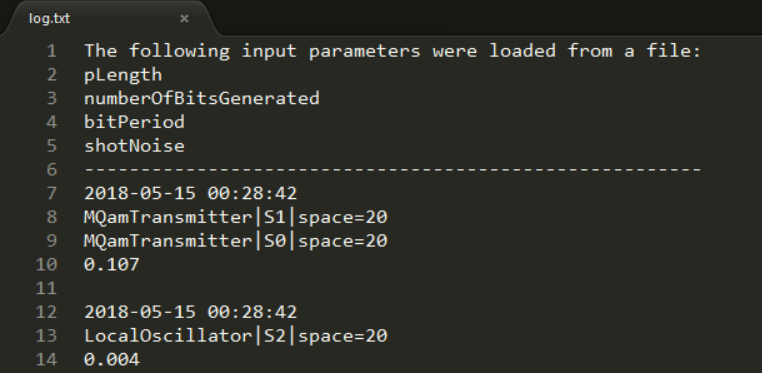
\includegraphics[width=.50\linewidth]{./chapter/simulator_structure/figures/logfile_input_parameters_changed}
\caption{Four input parameters where loaded from a file}
\label{fig:changedinputparameters}
\end{figure}

\subsection{Testing Log File}
In directory \textit{doc/tex/chapter/simulator\_structure/test\_log\_file/bpsk\_system/} there is a copy of the BPSK system. You may use it to test the Log File. The main method is located in file \textit{bpsk\_system\_sdf.cpp}

% bibliographic references for the section ----------------------------
\clearpage
\printbibliography[heading=subbibliography]
\end{refsection}
\addcontentsline{toc}{subsection}{Bibliography}
% ---------------------------------------------------------------------
\section{Input Parameters System}
\subsection{Introduction}
With the Input Parameters System (IPS) it is possible to read the input parameters from a file.

\subsubsection{Format Of The Input File}
In Figure \ref{fig:ipsfilecontent}, it is possible to observe the contents of the file \textbf{input\_parameters\_0.txt} used to load the values of some of the BPSK system's input parameters. The input file must respect the following properties:
\begin{enumerate}
\item Input parameter values can be changed by adding a line in the following format: \textbf{paramName=newValue}, where \textbf{paramName} is the name of the input parameter and \textbf{newValue} is the value to be assigned.
\item IPS supports scientific notation. This notation works for the lower case character \textbf{e} and the upper case character \textbf{E}.
\item If an input parameters is assigned the wrong type of value, method $\textbf{readSystemInputParameters()}$ will throw an exception.
\item Not all input parameters need to be changed.
\item The IPS supports comments in the form of the characters \textbf{//}. The comments will only be recognized if placed at the beginning of a line.
\end{enumerate}

\begin{figure}[H]
\centering
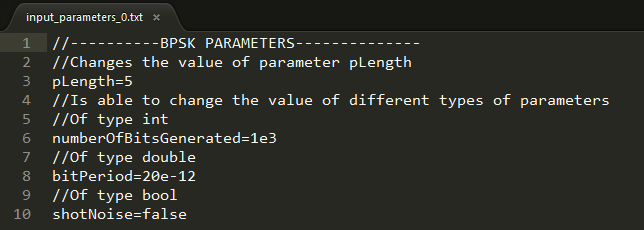
\includegraphics[width=0.8\linewidth]{./chapter/simulator_structure/figures/ips_input_file}
\caption{Content of file input\_parameters\_0.txt}
\label{fig:ipsfilecontent}
\end{figure}
\pagebreak
\subsubsection{Loading Input Parameters From A File}
Execute the following command in the Command Line:
\begin{itemize}
  \item[] \textbf{.\textbackslash{}some\_system.exe <input\_file\_path> <output\_directory>}
\end{itemize}
\
where \textbf{some\_system.exe} is the name of the executable generated after compiling the project, \textbf{<input\_file\_path>} is the path to the file containing the new input parameters; \textbf{<output\_directory>} is the directory where the output signals will be written into.

\subsection{How To Include The IPS In Your System}
In this illustrative example, the code of the BPSK System will be used. To implement the IPS the following requirements must be met:
\begin{enumerate}
\item Your system must include \textbf{netxpto\_20180418.h} or later.
\item A class that will contain the system input parameters must be created. This class must be a derived class of \textbf{SystemInputParameters}. In this case the created class is called \textbf{BPSKInputParameters}.
\item The created class must have 2 constructors. The implementation of these constructors is the same as \textbf{BPSKInputParameters}.
\begin{lstlisting}
BPSKInputParameters();
BPSKInputParameters(int argc, char*argv[]);
\end{lstlisting}
\item The created class must contain the method \textbf{initializeInputParameterMap()}. For every input parameter \textbf{addInputParameter(paramName,paramAddress)} must be called, where \textbf{paramName} is a string that represents the name of your input parameter and \textbf{paramAddress} is the address of your input parameter.
\begin{lstlisting}
void initializeInputParameterMap(){
	//Add parameters
}
\end{lstlisting}
\item All signals must be instantiated using the constructor that takes as argument, the file name and the folder name, according to the type of signal.
\begin{lstlisting}
Binary S0("S0.sgn", param.getOutputFolderName()) //S0 is a Binary signal
\end{lstlisting}
\item Method \textbf{main} must receive the following arguments.
\begin{lstlisting}
int main(int argc, char*argv[]){...}
\end{lstlisting}
\item The MainSystem must be instantiated using the following line of code. The \dots represent the list of blocks.
\begin{lstlisting}
System MainSystem{ vector<Block*> {...},param.getOutputFolderName(),param.getLoadedInputParameters()};
\end{lstlisting}
\end{enumerate}
\
The following code represents the input parameters class, \textbf{BPSKInputParameters}, and must be changed according to the system you are working on.
%%%%%%%%%%%%%%%%%%%%%%%%%%%CODE%%%%%%%%%%%%%%%%%%%%%%%%%%%%%%%%
\begin{lstlisting}
class BPSKInputParameters : public SystemInputParameters {
public:
	//INPUT PARAMETERS
	int numberOfBitsReceived{ -1 };
	int numberOfBitsGenerated{ 1000 };
	int samplesPerSymbol = 16;
    (...)

	/* Initializes default input parameters */
	BPSKInputParameters() : SystemInputParameters() {
		initializeInputParameterMap();
	}

	/* Initializes input parameters according to the program arguments */
    /* Usage: .\bpsk_system.exe <input_parameters.txt> <output_directory> */
	BPSKInputParameters(int argc, char*argv[]) : SystemInputParameters(argc,argv) {
		initializeInputParameterMap();
		readSystemInputParameters();
	}

	//Each parameter must be added to the parameter map by calling addInputParameter(string,param*)
	void initializeInputParameterMap(){
		addInputParameter("numberOfBitsReceived", &numberOfBitsReceived);
		addInputParameter("numberOfBitsGenerated", &numberOfBitsGenerated);
		addInputParameter("samplesPerSymbol", &samplesPerSymbol);
        (...)
	}
};
\end{lstlisting}
The method \textbf{main} should look similar to the following code.
\begin{lstlisting}
int main(int argc, char*argv[]){

    BPSKInputParameters param(argc, argv);

    //Signal Declaration and Initialization
    Binary S0("S0.sgn", param.getOutputFolderName());
	S0.setBufferLength(param.bufferLength);

	OpticalSignal S1("S1.sgn", param.getOutputFolderName());
	S1.setBufferLength(param.bufferLength);
    (...)

    //System Declaration and Initialization
	System MainSystem{ vector<Block*> { &B1, &B2, &B3, &B4, &B5, &B6, &B7, &B8},param.getOutputFolderName(),param.getLoadedInputParameters()};

    //System Run
	MainSystem.run();

	return 0;
}
\end{lstlisting}
%%%%%%%%%%%%%%%%%%%%%%%%%%%%%%%%%%%%%%%%%%%%%%%%%%%%%%%%%%%%%%%%%%%%%%
\pagebreak
The class \textbf{SystemInputParameters}, has the following constructors and methods available:
\begin{table}[H]
\centering
\begin{tabulary}{1.0\textwidth}{|p{5cm}|p{10cm}|}
\hline
\multicolumn{2}{|c|}{ \textbf{SystemInputParameters - Constructors} } \\
\hline
\textbf{Constructors}                   & \textbf{Comments} \\ \hline
SystemInputParameters()                        & Creates an object of SystemInputParameters with the default input parameters' values\\ \hline
SystemInputParameters(int argc, char*argv[])   & Creates an object of SystemInputParameters and loads the values according to the program arguments passed in the command line\\ \hline
\end{tabulary}
\end{table}

\begin{table}[H]
\centering
\begin{tabulary}{1.0\textwidth}{|p{9cm}|p{1cm}|p{5cm}|}
\hline
\multicolumn{3}{|c|}{ \textbf{SystemInputParameters - Methods} } \\
\hline
\textbf{Method}                                      & \textbf{Type} & \textbf{Comments} \\ \hline
addInputParameter(string name, int* variable)        & void          & Adds an input parameter whose value is of type int\\ \hline
addInputParameter(string name, double* variable)     & void	         & Adds an input parameter whose value is of type double\\ \hline
addInputParameter(string name, bool* variable)       & void	         & Adds an input parameter whose value is of type bool\\ \hline
readSystemInputParameters()                          & void	         & Reads the input parameters from a file.\\ \hline
\end{tabulary}
\end{table}

\cleardoublepage 